We use the same model and architecture as GPT-2 \cite{radford2019language}, including the modified initialization, pre-normalization, and reversible tokenization described therein, with the exception that we use alternating dense and locally banded sparse attention patterns in the layers of the transformer, similar to the Sparse Transformer \cite{child2019generating}. To study the dependence of ML performance on model size, we train 8 different sizes of model, ranging over three orders of magnitude from 125 million parameters to 175 billion parameters, with the last being the model we call GPT-3.  Previous work \cite{kaplan2020scaling} suggests that with enough training data, scaling of validation loss should be approximately a smooth power law as a function of size; training models of many different sizes allows us to test this hypothesis both for validation loss and for downstream language tasks.



\begin{table}
    
    \begin{adjustwidth}{-.8in}{-.8in}
    \begin{center}
        
        \begin{tabular}{l c c c c c c c}
        \toprule
        Model Name & $n_{\mathrm{params}}$ & $n_{\mathrm{layers}}$ & $d_{\mathrm{model}}$ & $n_{\mathrm{heads}}$ & $d_{\mathrm{head}}$  & Batch Size & Learning Rate \\
        \midrule
GPT-3 Small & 125M & 12 & 768 & 12 & 64 & 0.5M & $6.0 \times 10^{-4}$ \\                              
GPT-3 Medium & 350M & 24 & 1024 & 16 & 64 & 0.5M & $3.0 \times 10^{-4}$ \\                             
GPT-3 Large & 760M & 24 & 1536 & 16 & 96 & 0.5M & $2.5 \times 10^{-4}$ \\                             
GPT-3 XL & 1.3B & 24 & 2048 & 24 & 128 & 1M & $2.0 \times 10^{-4}$ \\                            
GPT-3 2.7B   & 2.7B & 32 & 2560 & 32 & 80 & 1M & $1.6 \times 10^{-4}$ \\                             
GPT-3 6.7B   & 6.7B & 32 & 4096 & 32 & 128 & 2M & $1.2 \times 10^{-4}$ \\                            
GPT-3 13B  & 13.0B & 40 & 5140 & 40 & 128 & 2M & $1.0 \times 10^{-4}$ \\                           
GPT-3 175B or ``GPT-3'' & 175.0B & 96 & 12288 & 96 & 128 & 3.2M & $0.6 \times 10^{-4}$ \\
        \bottomrule
        \end{tabular}
    \end{center}
    \end{adjustwidth}
    \caption{Sizes, architectures, and learning hyper-parameters (batch size in tokens and learning rate) of the models which we trained. All models were trained for a total of 300 billion tokens.}
    \label{table:param}
\end{table}

Table \ref{table:param} shows the sizes and architectures of our 8 models.  Here $n_{\mathrm{params}}$ is the total number of trainable parameters, $n_{\mathrm{layers}}$ is the total number of layers, $d_{\mathrm{model}}$ is the number of units in each bottleneck layer (we always have the feedforward layer four times the size of the bottleneck layer, $d_{\mathrm{ff}}$ $= 4 \ast d_{\mathrm{model}}$), and $d_{\mathrm{head}}$ is the dimension of each attention head.  All models use a context window of $n_{\mathrm{ctx}}=2048$ tokens.  We partition the model across GPUs along both the depth and width dimension in order to minimize data-transfer between nodes. The precise architectural parameters for each model are chosen based on computational efficiency and load-balancing in the layout of models across GPU’s.  Previous work \cite{kaplan2020scaling} suggests that validation loss is not strongly sensitive to these parameters within a reasonably broad range.

\begin{figure}
\centering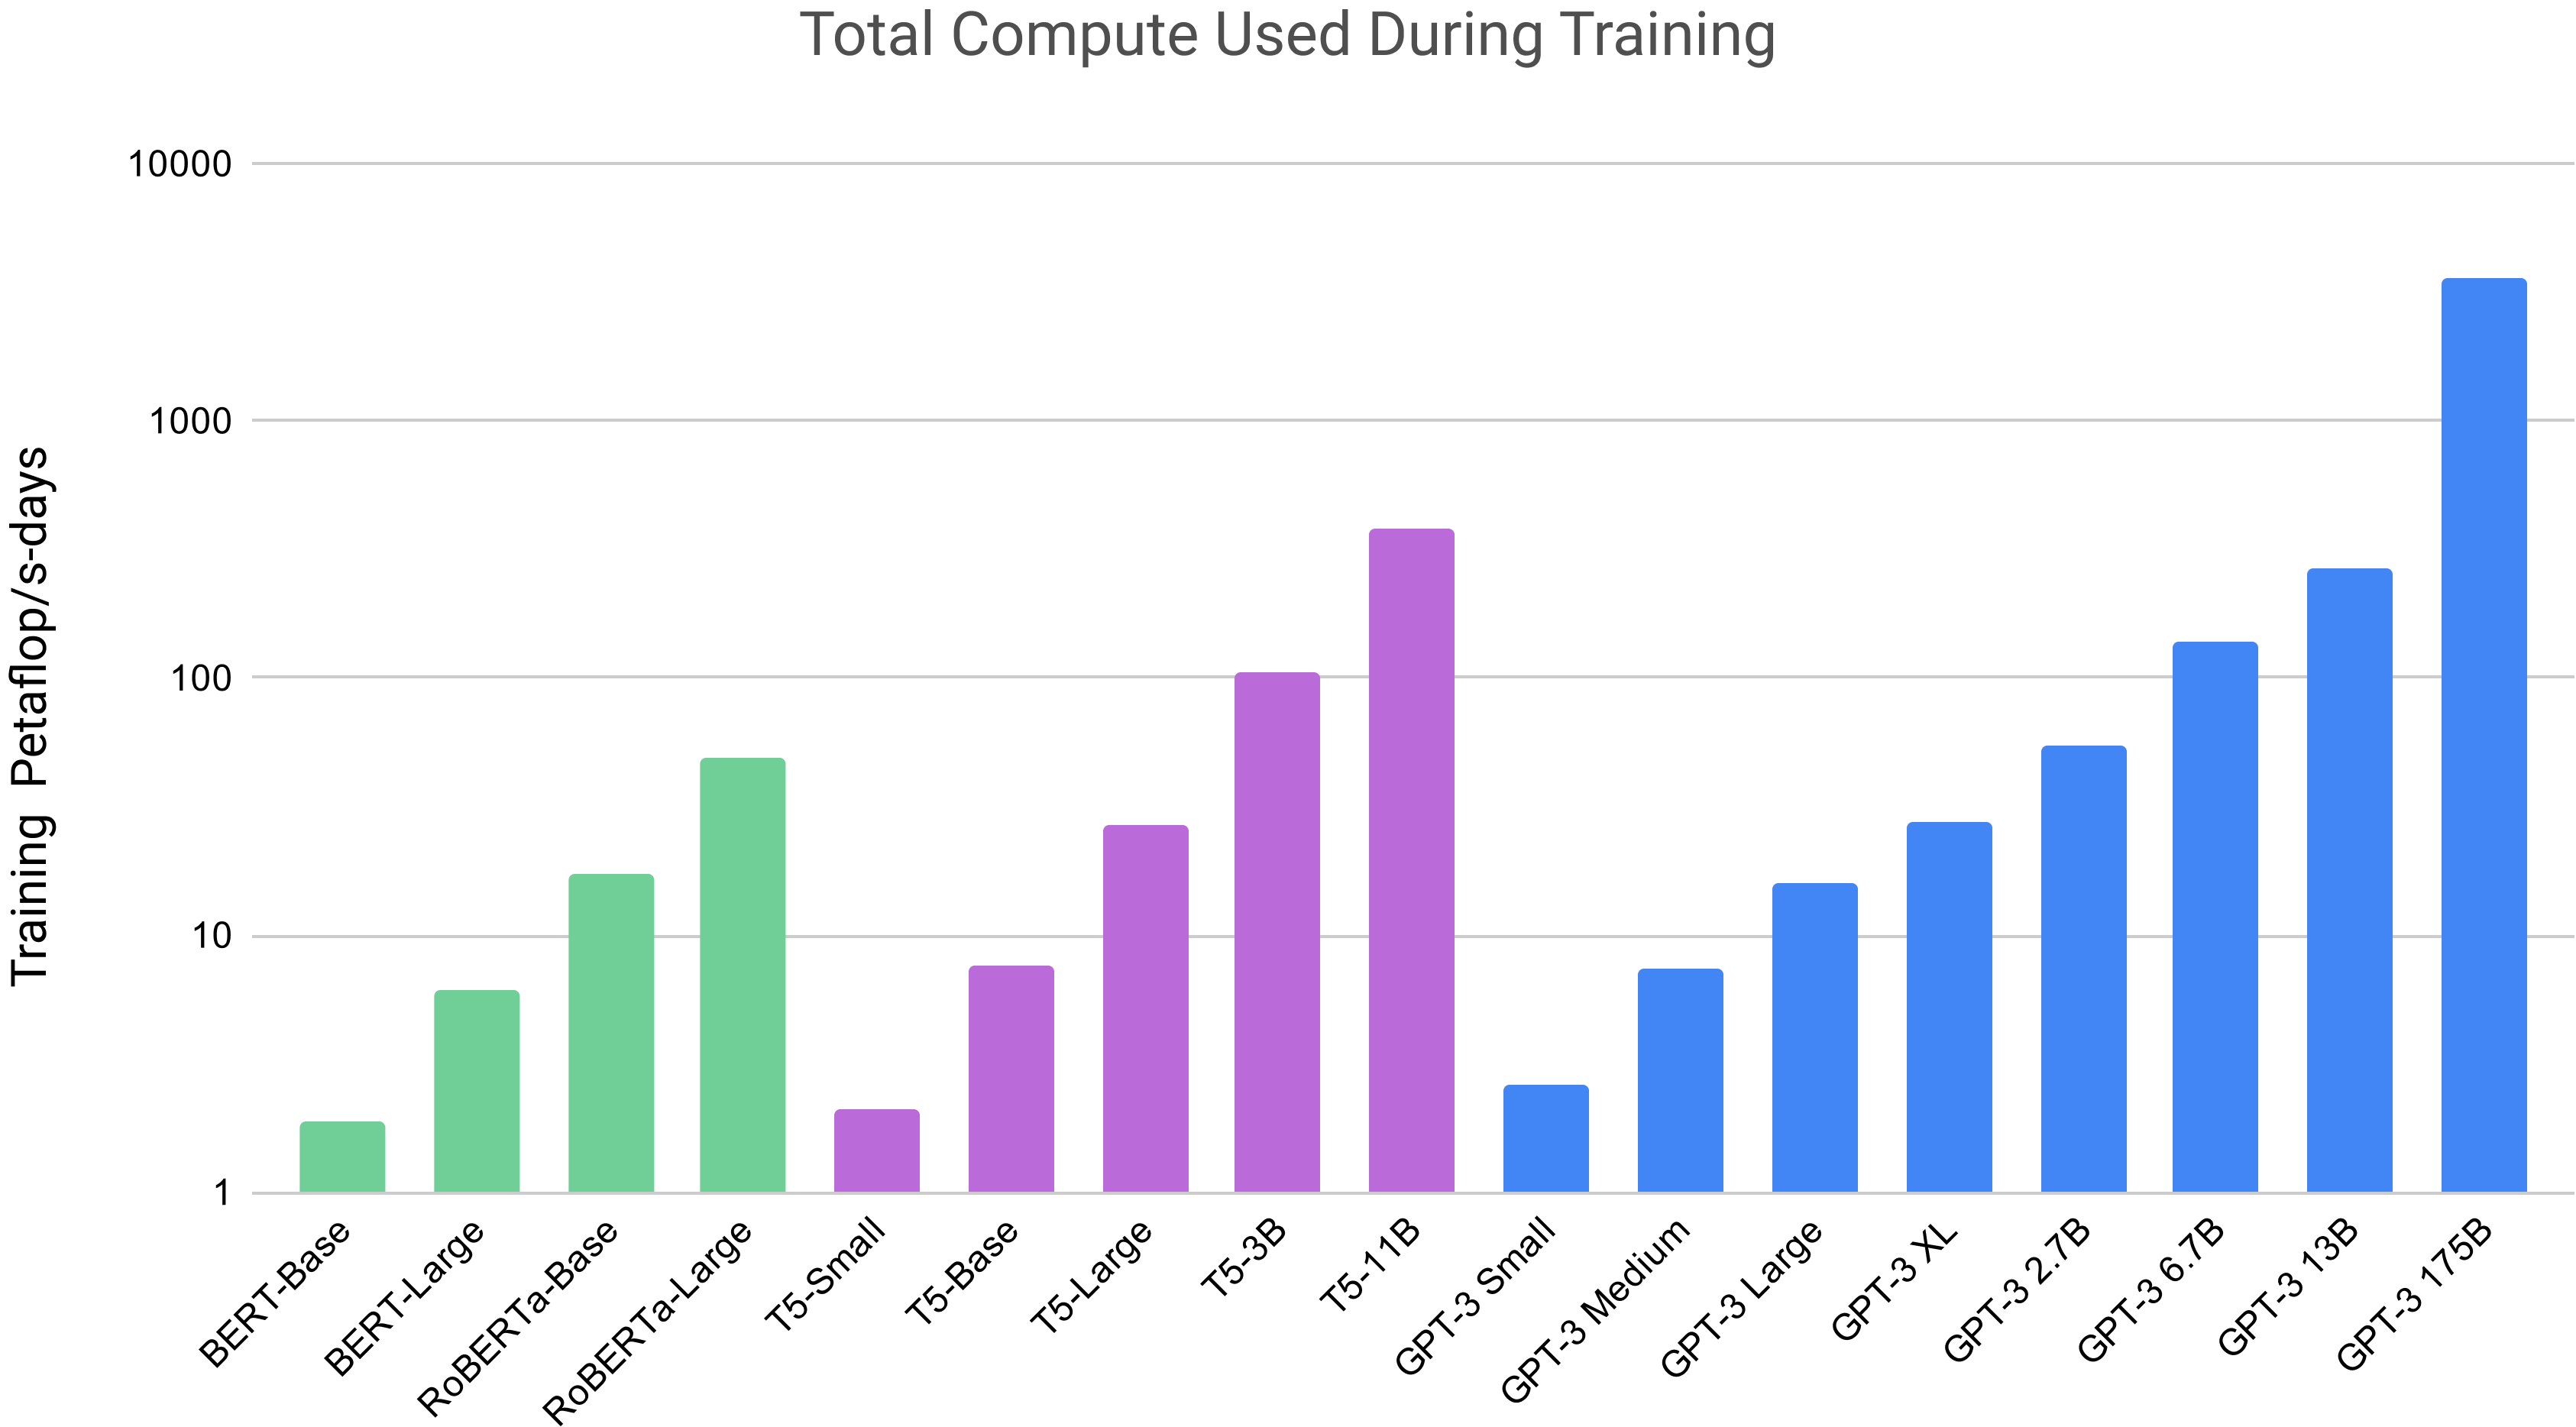
\includegraphics[width=0.9\linewidth]{figures/training_flops.png}
\caption{\textbf{Total compute used during training}. Based on the analysis in Scaling Laws For Neural Language Models \cite{kaplan2020scaling} we train much larger models on many fewer tokens than is typical. As a consequence, although GPT-3 3B is almost 10x larger than RoBERTa-Large (355M params), both models took roughly 50 petaflop/s-days of compute during pre-training. Methodology for these calculations can be found in Appendix \ref{appendix:total_compute_calculations}.
}
\label{figure:training flops}
\end{figure}
